\documentclass[border=10pt]{standalone}
\usepackage{pgfplots}
\pgfplotsset{compat=1.18}

\begin{document}
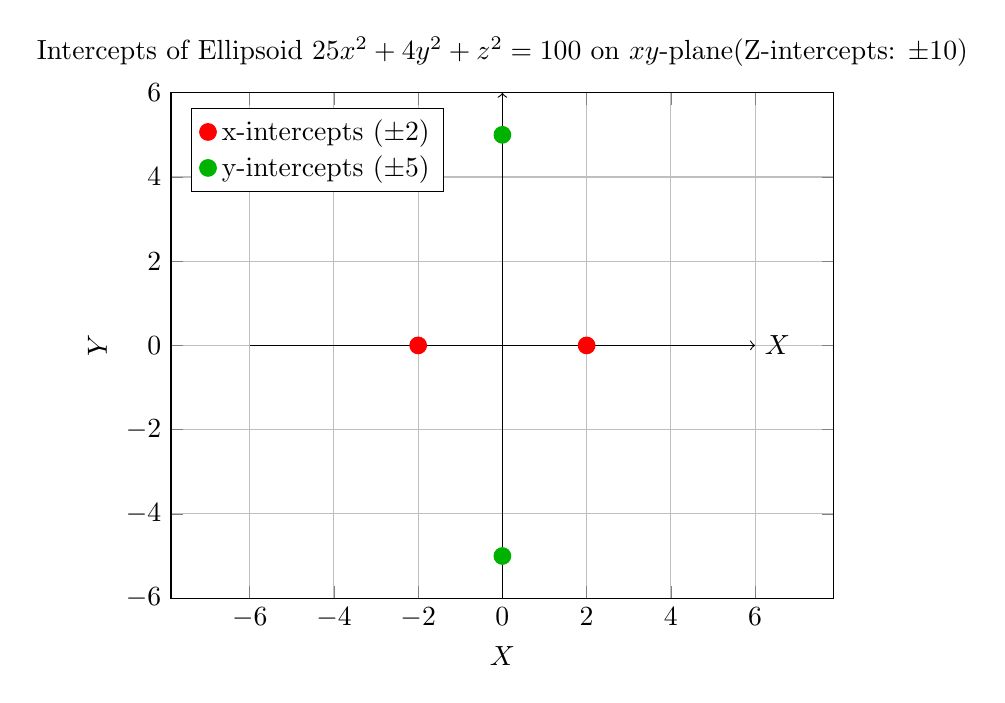
\begin{tikzpicture}
\begin{axis}[
    xlabel={$X$},
    ylabel={$Y$},
    title={Intercepts of Ellipsoid $25x^2 + 4y^2 + z^2 = 100$ on $xy$-plane\\(Z-intercepts: $\pm 10$)},
    axis equal,
    width=10cm,
    height=8cm,
    grid=major,
    xmin=-6, xmax=6,
    ymin=-6, ymax=6,
    legend pos=north west,
]
    % x-intercepts: (2, 0) and (-2, 0)
    \addplot[only marks, mark=*, mark size=3pt, color=red] coordinates {(2, 0) (-2, 0)};
    \addlegendentry{x-intercepts ($\pm 2$)}
    
    % y-intercepts: (0, 5) and (0, -5)
    \addplot[only marks, mark=*, mark size=3pt, color=green!70!black] coordinates {(0, 5) (0, -5)};
    \addlegendentry{y-intercepts ($\pm 5$)}
    
    % Draw axes lines for clarity
    \draw[->] (axis cs:-6,0) -- (axis cs:6,0) node[right] {$X$};
    \draw[->] (axis cs:0,-6) -- (axis cs:0,6) node[above] {$Y$};
    
\end{axis}
\end{tikzpicture}
\end{document}